\section{Celda Universal}

En esta secci\'on se analizan celdas de configuraciones diferentes que est\'an compuestas por dos integradores, con la finalidad de realizar un filtro $rechaza$  $banda$ que cumpla las siguientes especificaciones:

	\begin{table}[h!]
	\centering
	\begin{tabular}{c c}
		\hline
		$f_\infty$ & $51kHz$ \\ 
		notch depth &  $\geq 50dB$\\
		$\Delta f_a$ & $600Hz$\\
		$\Delta f_p$ & $880Hz$\\
		$A_a$ & $40dB$\\
		$A_p$ & $6dB$\\
		$G$ & $[-3:3]dB$\\
		$|Zin(f)|$ & $\geq 50k\Omega$\\		
		\hline
	\end{tabular}
	\caption{Especificaciones del filtro rechaza banda a realizar.}
	\label{especificaciones}
\end{table}

\subsection{Introducci\'on te\'orica}

Se comienza analizando el comportamiento de circuitos compuestos por dos integradores, representandolos mediante diagramas en bloques. El siguiente diagrama de la figura \ref{int1}\footnote{Adaptaci\'on de una imagen obtenida de: https://elxcompacme.files.wordpress.com/2014/03/filter-kendell-su.pdf} es una representaci\'on simple que permite entender lo que se desarrolla luego.

\begin{figure}[H] %!ht
	\centering
	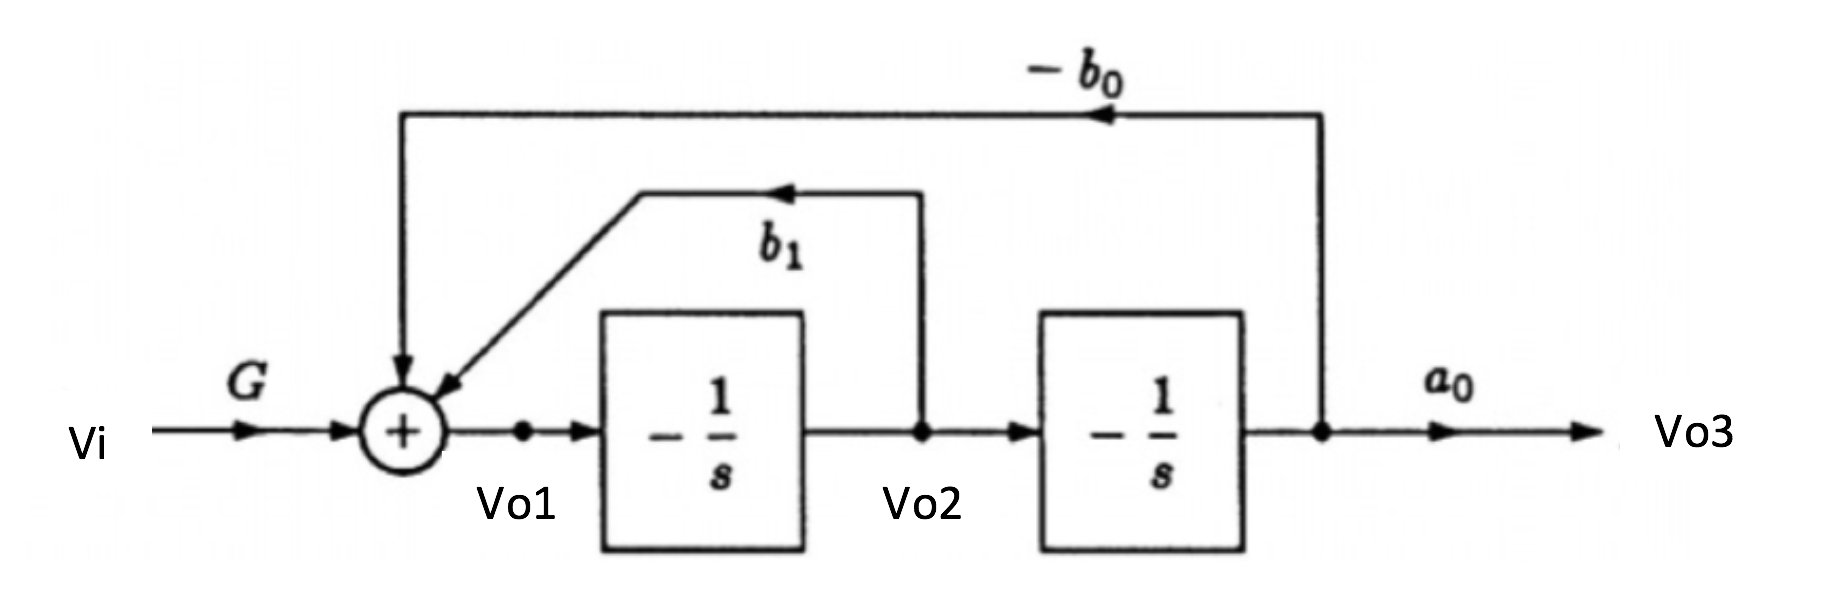
\includegraphics[width=12cm,height=12cm,keepaspectratio]{../EJ4/imagenes/int1.png}
	\caption{Representaci\'on en bloques de un circuito simple de segundo orden formado por dos integradores.}
	\label{int1}
\end{figure}

Del diagrama anterior, se obtienen las siguientes expresiones, a partir de las cuales se puede apreciar que se trata de un circuito de orden 2.

\begin{equation}
\begin{cases}
	Vo_2 = -\frac{1}{2} \cdot Vo_1\\
	Vo_3 = -\frac{1}{2} \cdot Vo_2\\
	H(s) = \frac{Vo_3}{V_i} = G \cdot \frac{a_0}{s^2 + b_1 s + b_0}
	\label{int2eq}
\end{cases}
\end{equation}

Si ahora se suman a la salida las tensiones $Vo_1$ y $Vo_2$ como se muestra en el diagrama de la siguiente figura \ref{int2}:

\begin{figure}[H] %!ht
	\centering
	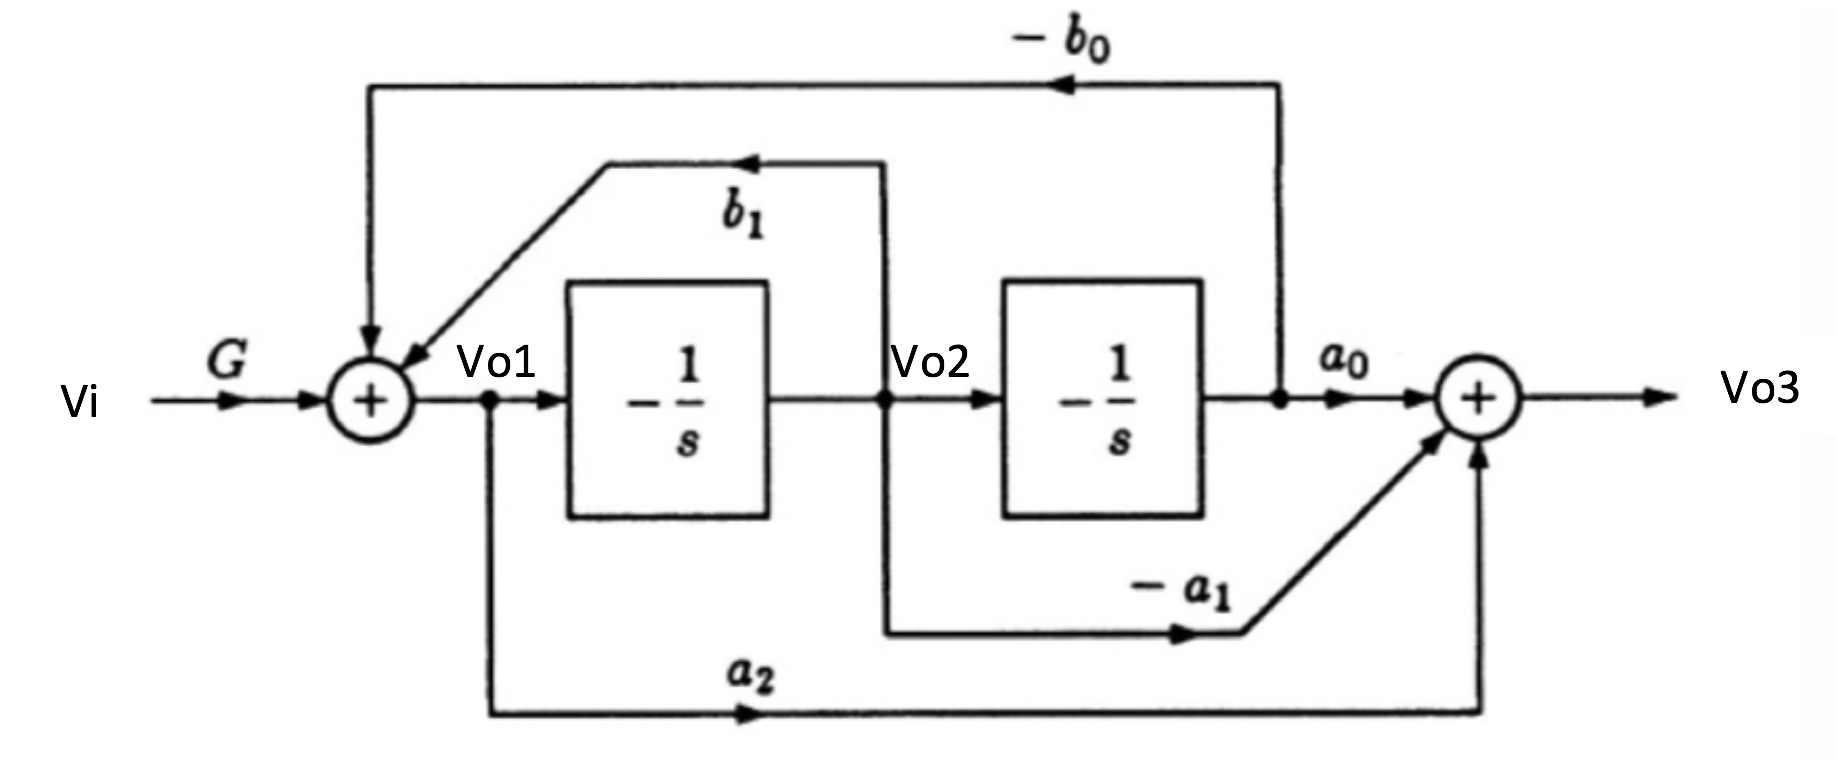
\includegraphics[width=12cm,height=12cm,keepaspectratio]{../EJ4/imagenes/int2.png}
	\caption{Misma representaci\'on en bloques que antes pero sumando las tensiones $Vo_1$ y $Vo_2$ a la salida.}
	\label{int2}
\end{figure}

As\'i se obtiene:

\begin{equation}
	\frac{Vo_3}{Vi} = G \cdot \frac{a_2s^2+a_1s+a_0}{s^2+b_1s+b_0}
	\label{int2eq}
\end{equation}

Las configuraciones que se analizan a continuaci\'on est\'an basadas en modificaciones sobre este \'ultimo diagrama de la figura \ref{int2} y su ecuaci\'on correspondiente \ref{int2eq}

\subsection{Configuraciones correspondientes a distintas celdas universales}

\todo{citar la pagina esta de internet}
\footnote{https://elxcompacme.files.wordpress.com/2014/03/filter-kendell-su.pdf}
\subsubsection{Kerwin-Huelsman-Newcomb (KHN)}

La siguiente es la celda Kerwin-Huelsman-Newcomb, tambi\'en llamada KHN por sus siglas. 

\begin{figure}[H] %!ht
	\centering
	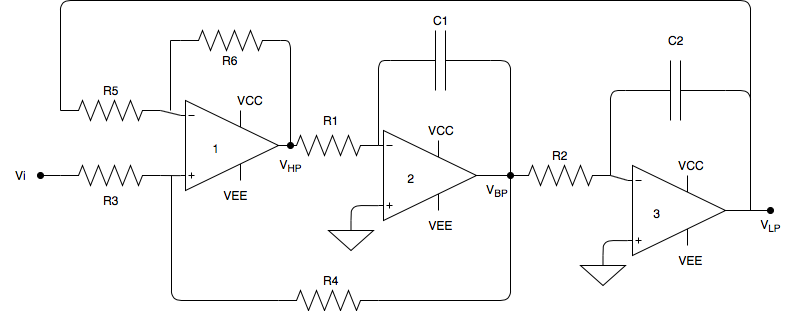
\includegraphics[width=12cm,height=12cm,keepaspectratio]{../EJ4/imagenes/KERWIN.png}
	\caption{Circuito Kerwin-Huelsman-Newcomb}
	\label{kerwin}
\end{figure}

\begin{table}[h!]
	\centering
	\begin{tabular}{c c c c c}
		Salida & $H(s)$ & $G$ & $\omega_0$ & $Q$\\
		\hline \\
		LP & $\frac{\frac{R_4}{R_5R_1R_2C_1C_2}\cdot \frac{R_5+R_6}{R_3+R_4}}{S^2+\frac{R_3}{R_5R_1C_1}\cdot \frac{R_5+R_6}{R_3+R_4}s+\frac{R_6}{R_5R_1R_2C_1C_2}}$& $\frac{R_4 (R_5+R_6)}{R_6(R_3+R_4)}$& \multirow{7}{*}{$\sqrt{\frac{R_4 (R_5+R_6)}{R_6(R_3+R_4)}}$}&
		\multirow{7}{*}{$\frac{R_5(R_3+R_4)}{R_3(R_5+R_6)}\cdot \sqrt{\frac{R_6R_1C_1}{R_5R_2C_2}}$}\\ \\
		BP & $- \frac{\frac{R_4}{R_5R_1C_1}\cdot \frac{R_5+R_6}{R_3+R_4} s}{S^2+\frac{R_3}{R_5R_1C_1}\cdot \frac{R_5+R_6}{R_3+R_4}s+\frac{R_6}{R_5R_1R_2C_1C_2}}$&$-\frac{R_4}{R_3}$& &\\ \\
		HP& $- \frac{\frac{R_4}{R_5}\cdot \frac{R_5+R_6}{R_3+R_4} S^2}{S^2+\frac{R_3}{R_5R_1C_1}\cdot \frac{R_5+R_6}{R_3+R_4}s+\frac{R_6}{R_5R_1R_2C_1C_2}}$& $\frac{R_4(R_5+R_6)}{R_5(R_3+R_4)}$& & \\ \\
		\hline
	\end{tabular}
	\caption{Caracter\'sticas de la celda Kerwin-Huelsman-Newcomb.}
	\label{hg_tt}
\end{table}

\begin{table}[h!]
	\centering
	\begin{tabular}{c c c c c c}
		  & $\omega_0$ & $Q$ &$G_{LP}$ & $G_{BP}$& $G_{HP}$\\
		\hline \\
	$R_1$ & $-\frac{1}{2}$& $\frac{1}{2}$ & $0$& $0$&$0$\\ \\
	$R_2$ & $-\frac{1}{2}$& $-\frac{1}{2}$ & $0$& $0$& $0$\\ \\
	$R_3$ & $0$& $-\frac{R_4}{R_3+R_4}$ & $-\frac{R_3}{R_3+R_4}$&$-1$ & $-\frac{R_3}{R_3+R_4}$\\ \\
	$R_4$ & $0$& $\frac{R_4}{R_3+R_4}$& $\frac{R_3}{R_3+R_4}$ &$1$ & $\frac{R_3}{R_3+R_4}$\\ \\
	$R_5$ & $-\frac{1}{2}$&$\frac{R_6-R_5}{2(R_5+R_6)}$ & $\frac{R_5}{R_5+R_6}$&$0$ & $-\frac{R_6}{R_5+R_6}$\\ \\
	$R_6$ & $\frac{1}{2}$& $-\frac{R_6-R_5}{2(R_5+R_6)}$ & $-\frac{R_5}{R_5+R_6}$& $0$&$\frac{R_6}{R_5+R_6}$ \\ \\
	$C_1$ & $-\frac{1}{2}$& $\frac{1}{2}$ & $0$& $0$&$0$ \\ \\
	$C_2$ & $-\frac{1}{2}$& $-\frac{1}{2}$ & $0$ & $0$&$0$\\ \\
		\hline
	\end{tabular}
	\caption{Sensibilidades de la celda Kerwin-Huelsman-Newcomb.}
	\label{sens_k}
\end{table}

Esta celda tiene sensibilidades bajas.

\begin{equation}
\begin{cases}
Vo_2 = -\frac{1}{2} \cdot Vo_1\\
Vo_3 = -\frac{1}{2} \cdot Vo_2\\
H(s) = \frac{Vo_3}{V_i} = G \cdot \frac{a_0}{s^2 + b_1 s + b_0}
\label{int2eq}
\end{cases}
\end{equation}

\todo{CHEQUEAR circuito porque en el palombo est\'a distinto!}

Dependiendo de d\'onde se tome la salida del circuito \ref{kerwin}, se puede obtener un filtro pasa altos, un pasa banda o un pasabajos. Lo que sucede con Kerwin-Huelsman-Newcomb es que no brinda una salida rechaza banda. La misma puede igual lograrse agregandole al circuito \ref{kerwin} un sumador, como se muestra en la figura \ref{sumador_extra}:

\begin{figure}[H] %!ht
	\centering
	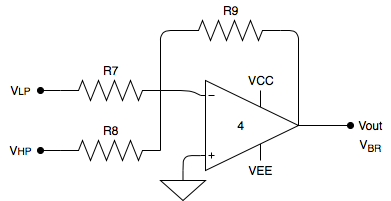
\includegraphics[width=8cm,height=8cm,keepaspectratio]{../EJ4/imagenes/sumador_extra.png}
	\caption{Sumador que se le agrega a la selda para obtener un rechaza banda.}
	\label{sumador_extra}
\end{figure}

\subsubsection{Tow-Thomas}

La celda Tow-Thomas var\'ia frente a la Kerwin-Huelsman-Newcomb al tener juntos a la entrada el sumador y el primer integrador, agregando luego un inversor y una resistencia en la realimentación que va de la salida $V_{LP}$ a la entrada del circuito. Esta nueva configuraci\'on, al igual que en la Kerwin-Huelsman-Newcomb sigue teniendo una salida de pasa bajos y una de pasa banda, pero ya no tiene una de pasa altos. Esto no importa en nuestro caso al querer obtener un rechaza bandas. Al igual que para el caso anterior, debe agregarse el sumador de la figura \ref{sumador_extra}.

\begin{figure}[H] %!ht
	\centering
	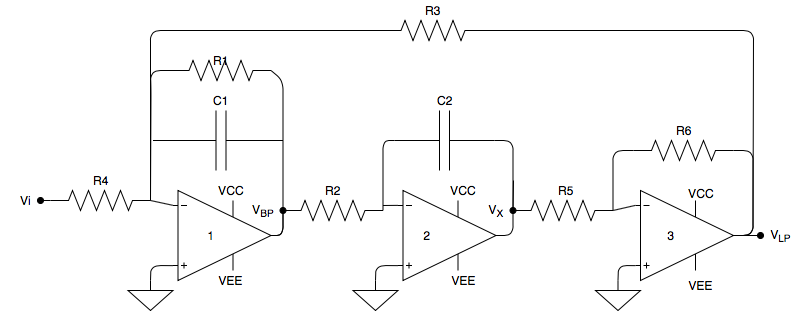
\includegraphics[width=12cm,height=12cm,keepaspectratio]{../EJ4/imagenes/TOW-THOMAS.png}
	\caption{Celda Tow-Thomas}
	\label{tow_thomas}
\end{figure}

Los par\'ametros correspondientes a la celda Tow-Thomas son los siguientes:


\begin{table}[h!]
	\centering
	\begin{tabular}{c c c c c}
		Salida & $H(s)$ & $G$ & $\omega_0$ & $Q$\\
		\hline \\
		LP & $-\frac{\frac{R_6/R_5}{R_2R_4C_1C_2}}{s^2+\frac{1}{R_1C_1}+\frac{R_6/R_5}{R_2R_3C_1C_2}}$& $- \frac{R_3}{R_4}$& \multirow{4}{*}{$\sqrt{\frac{R_6/R_5}{R_2R_3C_1C_2}}$}&
		\multirow{4}{*}{$\frac{R_1}{\sqrt{R_2R_3}}\sqrt{\frac{R_6C_1}{R_5C_2}}$}\\ \\
		BP & $-\frac{\frac{1}{R_4 C_1}s}{s^2+\frac{1}{R_1C_1}+\frac{R_6/R_5}{R_2R_3C_1C_2}}$&$-\frac{R_1}{R_4}$& &\\ \\
		\hline
	\end{tabular}
	\caption{Caracter\'isticas de la celda Tow-Thomas.}
	\label{hg_tt}
\end{table}

\begin{table}[h!]
	\centering
	\begin{tabular}{c c c c c }
		& $\omega_0$ & $Q$ &$G_{LP}$ & $G_{BP}$\\
		\hline \\
		$R_1$ & $0$& $1$ & $0$& $1$\\ \\
		$R_2$ & $-\frac{1}{2}$& $-\frac{1}{2}$ & $0$& $0$\\ \\
		$R_3$ & $-\frac{1}{2}$& $-\frac{1}{2}$ & $1$&$0$ \\ \\
		$R_4$ & $0$& $0$& $-1$ &$-1$ \\ \\
		$R_5$ & $-\frac{1}{2}$&$-\frac{1}{2}$ & $0$&$0$ \\ \\
		$R_6$ & $\frac{1}{2}$& $\frac{1}{2}$ & $0$& $0$ \\ \\
		$C_1$ & $-\frac{1}{2}$& $\frac{1}{2}$ & $0$& $0$\\ \\
		$C_2$ & $-\frac{1}{2}$& $-\frac{1}{2}$ & $0$ & $0$\\ \\
		\hline
	\end{tabular}
	\caption{Sensibilidades de la celda Tow-Thomas.}
	\label{sens_tt}
\end{table}


\subsubsection{Ackerberg-Mossberg}

\begin{figure}[H] %!ht
	\centering
	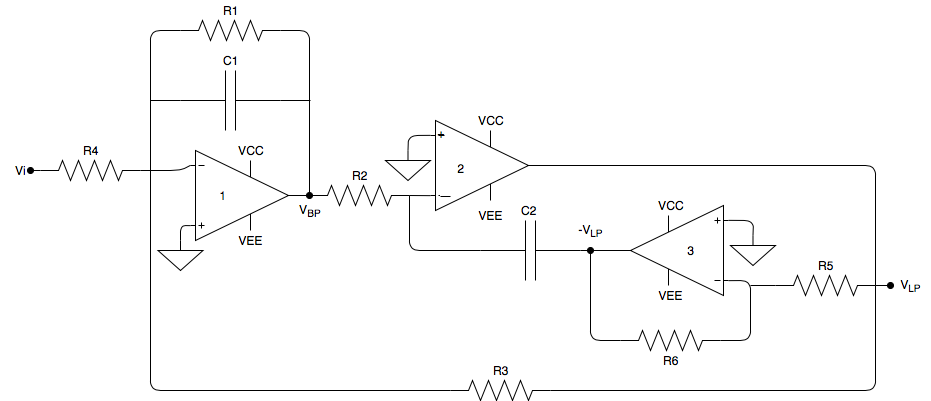
\includegraphics[width=12cm,height=12cm,keepaspectratio]{../EJ4/imagenes/ACKBERG.png}
	\caption{Celda Ackerberg-Mossberg}
	\label{ackerberg}
\end{figure}

\begin{table}[h!] %estas son las del libro!
	\centering
	\begin{tabular}{c c c c c}
		Salida & $H(s)$ & $G$ & $\omega_0$ & $Q$\\
		\hline \\
		LP & $- \frac{\frac{R_5}{C_1C_2R_2R_4R_6}}{s^2+\frac{1}{C_1R_1}s+\frac{R_5}{C_1C_2R_2R_3R_6}}$& $-\frac{R_3}{R_4}$& \multirow{4}{*}{$\sqrt{\frac{R_5}{C_1C_2R_2R_3R_6}}$}&
		\multirow{4}{*}{$C_1R_1\sqrt{\frac{R_5}{C_1C_2R_2R_3R_6}}$}\\ \\
		BP & $-\frac{\frac{1}{C_1R_4}s}{s^2+\frac{1}{C_1R_1}s + \frac{R_5}{C_1C_2R_2R_3R_6}}$&$-\frac{R_1}{R_4}$& &\\ \\
		\hline
	\end{tabular}
	\caption{Caracter\'isticas de la celda Ackerberg-Mossberg.}
	\label{am_tt}
\end{table}

\todo{chequear sensibilidad Q respecto a c1}
\begin{table}[h!]
	\centering
	\begin{tabular}{c c c c c }
		& $\omega_0$ & $Q$ &$G_{LP}$ & $G_{BP}$\\
		\hline \\
		$R_1$ & $0$ & $1$ & $0$ & $1$\\ \\
		$R_2$ & $-\frac{1}{2}$ & $-\frac{1}{2}$ & $0$ & $0$\\ \\
		$R_3$ & $-\frac{1}{2}$ & $-\frac{1}{2}$ & $1$ & $0$ \\ \\
		$R_4$ & $0$ & $0$ & $-1$ & $-1$ \\ \\
		$R_5$ & $\frac{1}{2}$ & $\frac{1}{2}$ & $0$ & $0$ \\ \\
		$R_6$ & $-\frac{1}{2}$ & $-\frac{1}{2}$ & $0$ & $0$ \\ \\
		$C_1$ & $-\frac{1}{2} $ & $\frac{1}{2}$ & $0$ & $0$\\ \\
		$C_2$ & $-\frac{1}{2}$ & $-\frac{1}{2}$ & $0$ & $0$\\ \\
		\hline
	\end{tabular}
	\caption{Sensibilidades de la celda Ackerberg-Mossberg.}
	\label{sens_am}
\end{table}

\subsubsection{Fleischer-Tow}

Una caracter\'istica importante a remarcar de la selda Flesicher-Tow es que, a diferencia de las celdas anteriores, permite realizar cualquier tipo de filtro de segundo orden sin la necesidad de agregar otro amplificador operacional. Como se ha estudiado en trabajos pr\'acticos anteriores, el amplificador operacional tiene ciertas limitaciones para un circuito, debidas al slew rate, a la saturaci\'on, entre otras; por lo que es ventajoso el hecho de no tener que agregar un amplificador operacional para obtener un filtro rechaza banda.


\begin{figure}[H] %!ht
	\centering
	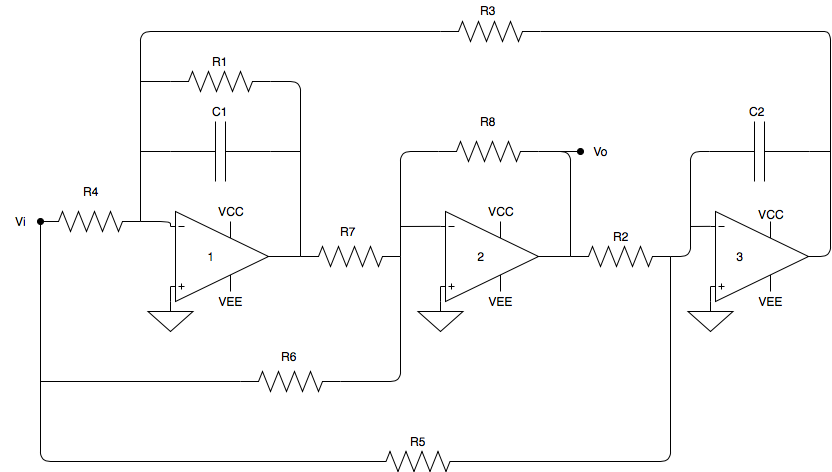
\includegraphics[width=12cm,height=12cm,keepaspectratio]{../EJ4/imagenes/FLEISCHER.png}
	\caption{Celda Fleischer-Tow}
	\label{fleischer}
\end{figure}

\begin{table}[h!] %estas son las del libro!
	\centering
	\begin{tabular}{c c c c}
		$H(s)$ gen\'erica & $\omega_0$ & $Q$\\
		\hline \\
		 $- \frac{\frac{R_8}{R_6}s^2+\left(\frac{R_8}{R_6R_1C_1}-\frac{R_8}{R_4R_7C_1}\right)s+\frac{R_8}{R_3R_5R_7C_1C_2}}{s^2+\frac{1}{R_1C_1}+\frac{R_8}{R_2R_3R_7C_1C_2}}$&$\sqrt{\frac{R_8}{R_2R_3R_7C_1C_2}}$&$R_1C_1\sqrt{\frac{R_8}{R_2R_3R_7C_1C_2}}$\\ \\
		\hline
	\end{tabular}
	\caption{Expresiones gen\'ericas de la celda Fleischer-Tow.}
	\label{f_generica}
\end{table}

\begin{table}[h!] %estas son las del libro!
	\centering
	\begin{tabular}{c c c c c c}
		Salida & Condiciones & $H(s)$ & $G$ & $\omega_0$ & $Q$\\
		\hline \\
		LP&$R_6=R_4=\infty$ &$- \frac{\frac{R_8}{R_3R_5R_7C_1C_2}}{s^2+\frac{1}{R_1C_1}+\frac{R_8}{R_2R_3R_7C_1C_2}}$& $-\frac{R_2}{R_5}$& \multirow{9}{*}{$\sqrt{\frac{R_8}{R_2R_3R_7C_1C_2}}$}&
		\multirow{9}{*}{$R_1C_1\sqrt{\frac{R_8}{R_2R_3R_7C_1C_2}}$}\\ \\
		BP &$R_6=R_5=\infty$  &$ \frac{\left(\frac{R_8}{R_4R_7C_1}\right)s}{s^2+\frac{1}{R_1C_1}+\frac{R_8}{R_2R_3R_7C_1C_2}}$&$\frac{R_1R_8}{R_4R_7}$& &\\ \\
		HP & $R_5=\infty$&\multirow{2}{*}{$- \frac{\frac{R_8}{R_6}s^2}{s^2+\frac{1}{R_1C_1}+\frac{R_8}{R_2R_3R_7C_1C_2}}$}&\multirow{2}{*}{$-\frac{R_8}{R_6}$}& &\\ 
		&$R_1R_6=R_4R_7$ & & & &\\ \\
		BR &$R_1R_6=R_4R_7$ &\multirow{2}{*}{$- \frac{\frac{R_8}{R_6}s^2+\frac{R_8}{R_3R_5R_7C_1C_2}}{s^2+\frac{1}{R_1C_1}+\frac{R_8}{R_2R_3R_7C_1C_2}}$}&\multirow{2}{*}{$-\frac{R_8}{R_6} = -\frac{R_5}{R_2}$}& &\\ 
		& $R_5R_8=R_2R_6$ & & & & \\ \\
		\hline
	\end{tabular}
	\caption{Caracter\'isticas de la celda Fleischer-Tow.}
	\label{f_cars}
\end{table}

\todo{ver sensibilidades Gbr}
\begin{table}[h!]
	\centering
	\begin{tabular}{c c c c c c c}
		& $\omega_0$ & $Q$ &$G_{LP}$ & $G_{BP}$& $G_{HP}$& $G_{BR}$\\
		\hline \\
		$R_1$ & $0$ & $1$ & $0$ & $1$ & $0$ & $0$\\ \\
		$R_2$ & $-\frac{1}{2}$ & $-\frac{1}{2}$ & $1$ & $0$ & $0$ & $-1$\\ \\
		$R_3$ & $-\frac{1}{2}$ & $-\frac{1}{2}$ & $0$ & $0$ & $0$ & $0$\\ \\
		$R_4$ & $0$ & $0$ & $0$ & $-1$ & $0$ & $0$\\ \\
		$R_5$ & $0$ & $0$ & $-1$ & $0$ & $0$ & $1$\\ \\
		$R_6$ & $0$ & $0$ & $0$ & $0$ & $-1$ & $-1$\\ \\
		$R_7$ & $-\frac{1}{2}$ & $-\frac{1}{2}$ & $0$ & $-1$ & $0$ & $0$\\ \\
		$R_8$ & $\frac{1}{2}$ & $\frac{1}{2}$ & $0$ & $1$ & $1$ & $1$\\ \\
		$C_1$ & $-\frac{1}{2}$ & $\frac{1}{2}$ & $0$ & $0$ & $0$ & $0$\\ \\
		$C_2$ & $-\frac{1}{2}$ & $-\frac{1}{2}$ & $0$ & $0$ & $0$ & $0$\\ \\
		\hline
	\end{tabular}
	\caption{Sensibilidades de la celda Fleischer-Tow}
	\label{sens_am}
\end{table}